%%%%%%%%%%%%%%%%%%%%%%%%%%%%%%%%%%%%%%%%%
% Short Sectioned Assignment
% LaTeX Template
% Version 1.0 (5/5/12)
%
% This template has been downloaded from:
% http://www.LaTeXTemplates.com
%
% Original author:
% Frits Wenneker (http://www.howtotex.com)
%
% License:
% CC BY-NC-SA 3.0 (http://creativecommons.org/licenses/by-nc-sa/3.0/)
%
%%%%%%%%%%%%%%%%%%%%%%%%%%%%%%%%%%%%%%%%%

%----------------------------------------------------------------------------------------
%	PACKAGES AND OTHER DOCUMENT CONFIGURATIONS
%----------------------------------------------------------------------------------------

\documentclass[paper=a4, fontsize=11pt]{scrartcl} % A4 paper and 11pt font size

\usepackage[T1]{fontenc} % Use 8-bit encoding that has 256 glyphs
\usepackage{fourier} % Use the Adobe Utopia font for the document - comment this line to return to the LaTeX default
\usepackage[english]{babel} % English language/hyphenation
\usepackage{amsmath,amsfonts,amsthm} % Math packages

\usepackage{sectsty} % Allows customizing section commands
\allsectionsfont{\centering \normalfont\scshape} % Make all sections centered, the default font and small caps

\usepackage{parskip}
\usepackage{fancyhdr} % Custom headers and footers
%\pagestyle{fancyplain} % Makes all pages in the document conform to the custom headers and footers
\fancyhead[L]{Tekin �zbek\\Benjamin Yan} % Empty left footer
\fancyhead[R]{COMP 4203 Project Report\\ An Implementation of Internet Networking Using XBee Modules} % Empty center footer
\fancyfoot[C]{\thepage} % Page numbering for right footer
\renewcommand{\headrulewidth}{0pt} % Remove header underlines
\renewcommand{\footrulewidth}{0pt} % Remove footer underlines
\setlength{\headheight}{5pt} % Customize the height of the header
\setlength{\parindent}{1cm} % Default is 15pt.

\usepackage{graphicx}
\usepackage{alltt}
\usepackage{subcaption}
\usepackage{url}
\usepackage{natbib}
\usepackage{tabulary}
\usepackage[toc,page]{appendix}

\numberwithin{equation}{section} % Number equations within sections (i.e. 1.1, 1.2, 2.1, 2.2 instead of 1, 2, 3, 4)
\numberwithin{figure}{section} % Number figures within sections (i.e. 1.1, 1.2, 2.1, 2.2 instead of 1, 2, 3, 4)
\numberwithin{table}{section} % Number tables within sections (i.e. 1.1, 1.2, 2.1, 2.2 instead of 1, 2, 3, 4)

\setlength\parindent{0pt} % Removes all indentation from paragraphs - comment this line for an assignment with lots of text

%----------------------------------------------------------------------------------------
%	TITLE SECTION
%----------------------------------------------------------------------------------------

\newcommand{\horrule}[1]{\rule{\linewidth}{#1}} % Create horizontal rule command with 1 argument of height

\title{	
\normalfont \normalsize 
\horrule{0.5pt} \\[0.4cm] % Thin top horizontal rule
\huge COMP 4203 Project Report\\ An Implementation of Internet Networking Using XBee Modules\\ % The assignment title
\horrule{2pt} \\[0.5cm] % Thick bottom horizontal rule
\large Tekin �zbek\\Benjamin Yan\\
\vspace{3cm}
\textbf{Disclaimer:} The work presented in this report is new, and prepared only for the course COMP 4203, Winter 2015, Carleton University.
}
\date{\normalsize\today} % Today's date or a custom date

\begin{document}

\begin{titlepage}
\clearpage
\maketitle % Print the title
\tableofcontents
%\thispagestyle{empty}
\end{titlepage}
\newpage

\section{Introduction}
%\setcounter{page}{1}

\subsection{Background}
The Internet is a well-established global system of computer networks, with a standard set of protocols that govern the communications and interactions between the connected computers and devices. The various devices and systems connected to the Internet are linked by a variety of technologies, ranging from electronic and wireless to optic networks \cite{wiki_internet}.

The Internet has become a crucial part of the everyday lives of most North Americans, and we rely on it for a variety of services and resources. Although there are many inexpensive off-the-shelf solutions to connect a personal computer or device to the Internet, we were interested in exploring the possibility of creating computer networks that communicate using the standard Internet protocol suite \cite{wiki_tcp_ip}, and are linked by an alternative method.

\subsection{Problem Definition}
Given the above information, we seek to develop a framework for building computer networks using XBee modules, which are small low-power radio transceivers designed to connect devices over short ranges \cite{digi_xbee}. There are a number of different models in the XBee family, each with different specifications in power, range, and compatibility; all XBee modules can either transmit raw radio signals, or communicate with each other using a packet-based application programming interface (API).

Our specific goal is to use two XBee modules to create a wireless point-to-point connection between two computers. Connection between each pair of computer and XBee module is established over USB, facilitated by a small circuit board that interfaces the XBee modules with the USB connector \cite{ftdichip}. To create an Internet connection between the computers, we use a TUN kernel device that simulates a network layer device and transmits network layer packets between the computer and XBee module \cite{wiki_tun_tap}. In other words, network layer packets are encapsulated in the XBee module packets, and an internet connection is virtualized between the two computers.

\subsection{Project Results}
Over the course of this project, we have developed a lightweight C++ program that allows us to establish a permanent wireless connection between two computers, using the XBee modules. The C++ program allows the two computers to address each other directly using IP addresses, and to communicate using standard network layer protocols to access / provide services for each other. This includes pinging over the network, establishing SSH connections, transmitting files over SFTP, and serving webpages.

To achieve these results, we designed our own data encapsulation scheme that encapsulates IP packets in one or more XBee packets, due to the small size limit of the XBee packets. Reading and writing data to the XBee modules was done through an open-source library called libxbee \cite{libxbee}. We had considered using data compression to decrease the transmission size, but this proved to be time-consuming, and provided no benefits. 

\subsection{Report Outline}

The remainder of the report is organized as follows: In Section~\ref{sec:background}, we present the background information about the various devices, protocols, and tools used in this project. In Section~\ref{sec:sys_details}, we describe the way that we have designed and implemented our system, the way that the XBee modules have been setup, and we discuss some examples of usage. In Section~\ref{sec:summary}, we give a brief summary of our achievements and conclude the paper.




\section{Detailed Background}
\label{sec:background}

In this section, we provide the reader with the detailed background knowledge required to understand:
\begin{itemize}
\item what an XBee module is.
\item what a TUN device is.
\item how we encapsulate IP packets from one computer to another, using the XBee packet API.
\end{itemize}

\subsection{XBee Modules}

The XBee family of wireless modules are small radio transceivers, developed and sold by Digi International \cite{wiki_xbee}. They are based on the IEEE 802.15.4 standard, which is designed for low power and low speed devices, and operate at about 10m ranges with speeds of around 250kbit/s, although many devices do not reach this speed \cite{wiki_ieee_802_15_4}. There are two types of network nodes under this standard: a full-function device (FFD), which, as the name suggests, has full functionality, and can act as ``PAN coordinators" in the network; and a reduced-ruction device (RFD), which are simpler devices that cannot act as coordinators.

\begin{figure}[ht]
\centering
  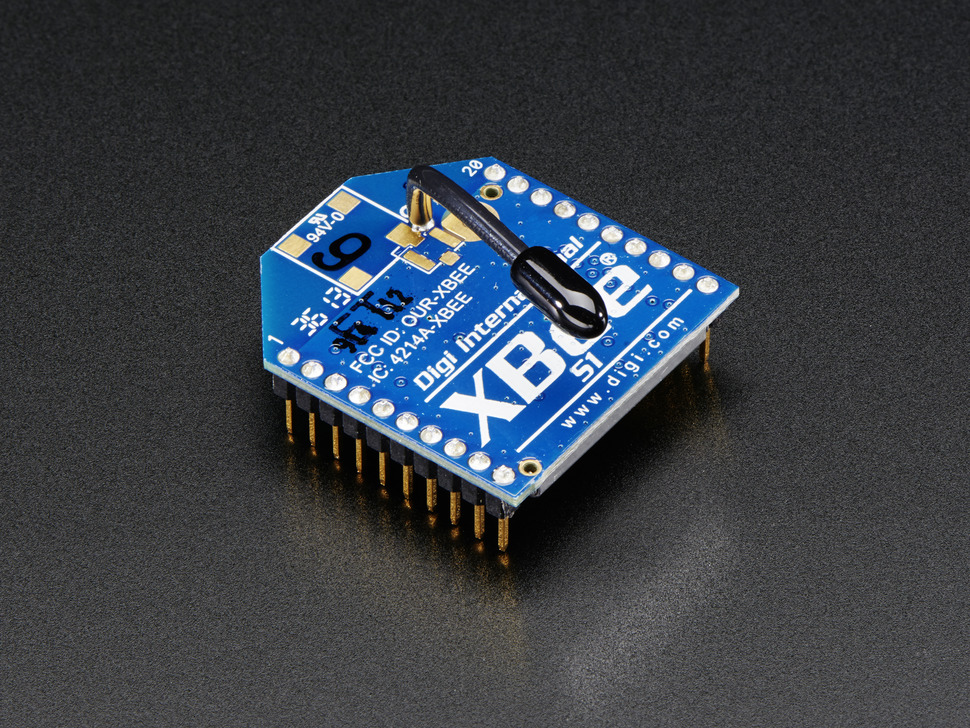
\includegraphics[width=.5\linewidth]{xbee.jpg}
  \captionof{figure}{Example of an XBee module}
  \label{fig:xbee}
\end{figure}

The standard allows the creation of two types of networks: a star network, where all communication between nodes is transmitted through a central Coordinator; or a peer-to-peer network, where nodes can communicate with each other directly \cite{wiki_ieee_802_15_4}. In either network type, at least one full-function device must act as a coordinator; multiple coordinators can also be networked together. Examples of these networks are shown in Figure~\ref{fig:ieee_802_15_topologies}.

\begin{figure}[ht]
\centering
  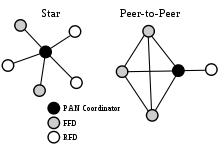
\includegraphics[width=.5\linewidth]{IEEE_802_15_4_Star_P2P.png}
  \captionof{figure}{Star and peer-to-peer topologies allowed by IEEE 802.15.4 \cite{wiki_ieee_802_15_4}}
  \label{fig:ieee_802_15_topologies}
\end{figure}

The XBee modules are full-function devices, so they can each act as a coordinator. Since we are working with only 2 devices, we arbitrarily choose one to be the coordinator, and set up a simple peer-to-peer network between the two devices. Although the manufacturer's specifications state that the RF line of sight range for many XBee models are on the order of kilometres, we have found that effective indoor distances, without data loss, are limited to a few metres. 

\begin{figure}[ht]
\centering
  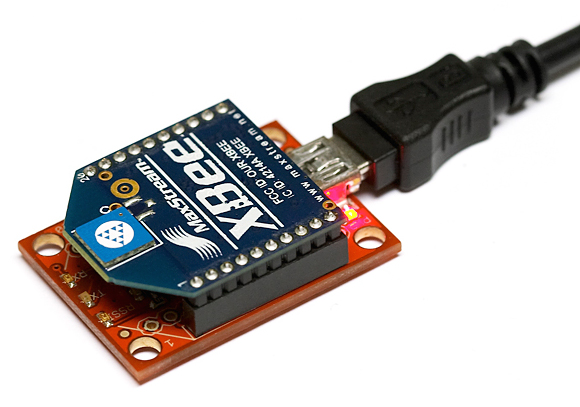
\includegraphics[width=.5\linewidth]{xbee_usb_adapter.jpg}
  \captionof{figure}{Example of a XBee USB adapter circuit}
  \label{fig:xbee_usb_adapter}
\end{figure}

To interface the XBee modules with computers, we have also obtained an USB adapter for each module, shown in figure~\ref{fig:xbee_usb_adapter} \cite{sparkfun_xbee_usb}. Interfacing with the module through a USB connection serves two purposes: first, we can configure the devices through the USB connection, and set parameters such as coordinator address, and baud rate;  this can be done using the X-CTU program from the XBee manufacturer (Figure~\ref{fig:xctu}). Second, we can send and receive data to the XBee modules over USB. Transmitting data over the usb device is particularly convenient in Linux systems, because we can easily read from and write to the USB device file \cite{wiki_device_file}. We were required to install the FTDI driver on the computers, so that the USB devices can be recognized \cite{ftdichip}.

\begin{figure}[ht]
\centering
  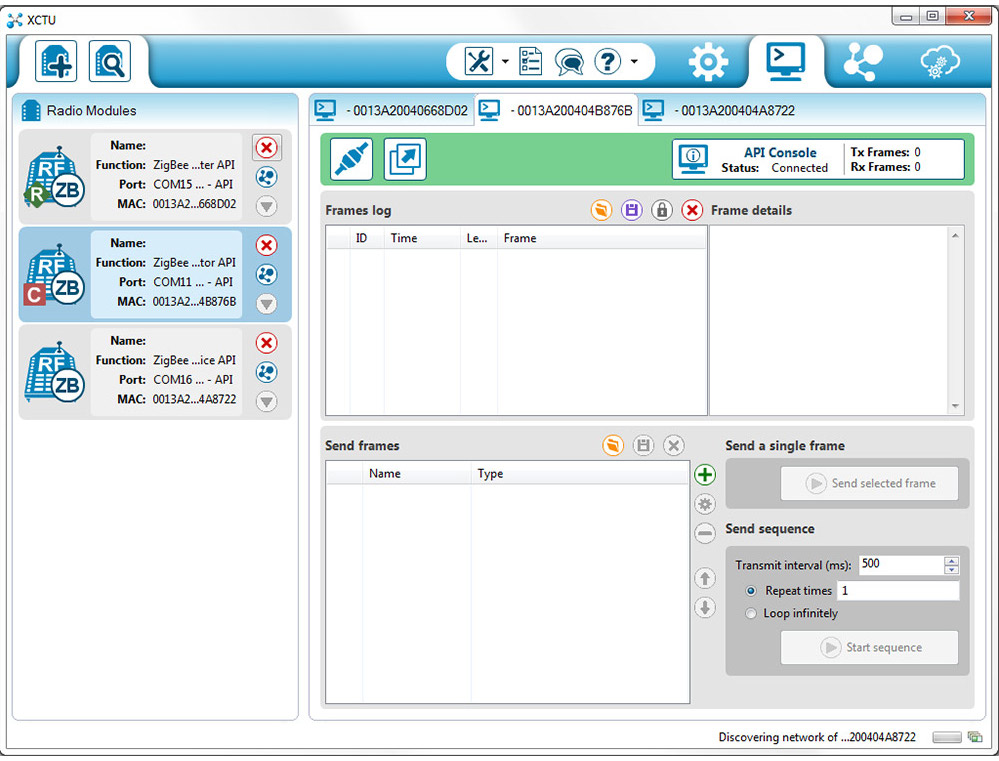
\includegraphics[width=.9\linewidth]{xctu.jpg}
  \captionof{figure}{X-CTU program interface for configuring XBee modules and networks \cite{digi_xctu}}
  \label{fig:xctu}
\end{figure}

Simply being able to transmit and receive data using the XBee modules is not enough for our objectives, however. Next, we discuss how we can virtualize the network layer using the XBee wireless connection, with TUN devices.

\subsection{TUN Devices}

A TUN device is a virtual network kernel device that simulates the network layer, and is treated in the same way as a network adapter, such as an Ethernet device \cite{wiki_tun_tap}. Once the TUN device is set up, a user-space program can be attached to the device. For our purposes, we can assign an IP address to the device, and enable it, using the Linux \textit{ip} command. This means that any time that the kernel refers to this IP address, data transmission is done through the user-space program, to the TUN device, instead of the Ethernet or wireless device on the computer \cite{backreference_tuntap}.

Similar to TUN devices are TAP devices, which stands for ``network tap" \cite{wiki_tun_tap}. The difference between a TUN device and a TAP device is in the layer: a TUN device works at the network layer, and transmits IP packets, while a TAP device works at the link layer, and transmits Ethernet frames \cite{backreference_tuntap}. Since we are interested in working directly with IP packets, we use TUN devices only, not TAP devices. We create a TUN device by opening a file under the path /dev/net/tun, and setting the file's flags for a TUN device.

\subsection{Data Encapsulation}
\subsubsection{XBee Fragments}
Although the IEEE 802.15.4 standard specifies a maximum packet size of 127 bytes, the XBee Series 2 modules that we are using only allows a maximum payload of 72 bytes, due to significant number of bytes used in the packet header \cite{digi_sending_data}. Since we are sending IP packets, which, for IPv4, have a size range between 20 and $65,535$ bytes \cite{wiki_ipv4}, it is very likely that one XBee fragment is not enough to contain the entire IP packet. Therefore, we need to be able to transmit a single IP packet over several XBee fragments.

\begin{figure}[ht]
\centering
  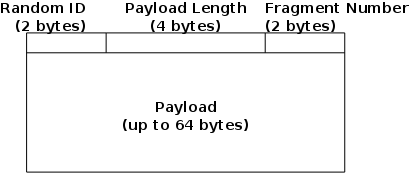
\includegraphics[width=.75\linewidth]{xbee_packet.png}
  \captionof{figure}{XBee fragment header and payload}
  \label{fig:xbee_packet}
\end{figure}

To do so, we have developed an encapsulation scheme for the 72byte XBee fragment, which contains a header portion and a payload portion, shown in Figure~\ref{fig:xbee_packet}. The first 2 bytes of the header is a randomly generated ID, unique for each IP packet transmitted. The next 4 bytes represent the length of the fragment payload. The following 2 bytes represent the fragment index number in the sequence for that IP packet. The remainder of the fragment contains the actual payload, which is a portion of the IP packet.

\begin{figure}[!ht]
\centering
  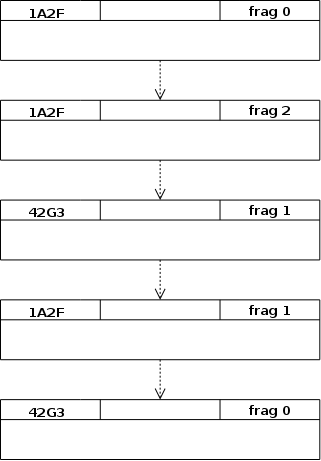
\includegraphics[width=.5\linewidth]{xbee_packets_out_of_order.png}
  \captionof{figure}{XBee fragments arriving out of order}
  \label{fig:xbee_packets_out_of_order}
\end{figure}

In the case that we transmit several IP packets, each packet over several XBee fragments, it is possible that the packets may arrive out of order. This is the reason that we employ a 2 byte ID number, and a 2 byte fragment number. Figure~\ref{fig:xbee_packets_out_of_order} shows a potential scenario where a number of fragments representing several different IP packets arrive out of order, and we must rely on the ID and fragment number to correctly construct the distinct IP packets.

\subsubsection{Wireless Security}
It should be noted here that our implementation does not contain any security features. Specifically, our design is highly susceptible to man-in-the-middle attacks. This type of attack could be carried out by an adversary who intercepts our radio transmissions, modifies the information, and sends the modified data. It is also possible for an adversary to simply forge XBee fragments, using valid headers and payload, and broadcast the fragments to our XBee modules.

To protect against this attack, we could use a secure encryption algorithm to encrypt the entire XBee fragment, and send the encrypted fragment. In this case, we already have a fragment number and a secret random ID inside the encrypted fragment, so the scheme would not be vulnerable to replay attacks. Alternatively, we could encrypt the IP packet, and send portions of the encrypted packet as payload in the XBee fragments. This method is less secure, because the header portion would be unencrypted, so an adversary could forge the header and perform a replay attack. In either case, we should also ensure the authenticity of each fragment by computing a message authentication code (MAC) for the fragment. This would consume additional bytes in each message.

Ultimately, we chose not to employ encryption in our design, because it would take up additional space in our already-limited fragment size. Since the goal of this project is only to explore the possibility of computer networking  using XBee modules, the security aspect is not as crucial. Additionally, due to the range limitations on the XBee modules, and the novelty in their use as a networking interface, it seems unlikely that an adversary could perform an attack undetected, under our noses.

\subsection{Summary}

In this section, we have discussed, in detail, the background information for XBee modules, TUN devices, and our method for encapsulating IP packets. Next, we discuss how we implemented our design, and provide examples of the system in use.



\section{System and Implementation Details}
\label{sec:sys_details}
In the previous section, we have provided the reader with the necessary background knowledge for each component of our project. Here, we present the details of the implementation and usage. In section~\ref{subsec:sys_description}, we discuss the details of the system design; in section~\ref{subsec:config}, we discuss the detailed configuration of the XBee modules; and in section~\ref{subsec:usage}, we provide examples of our system in use, over the network connection created between two computers.

\subsection{Description of the System}
\label{subsec:sys_description}

\subsubsection{Component Breakdown}

As mentioned in the previous section, we create a network connection between two computers, using XBee modules at the link layer. At the application level on each computer, the network is virtualized so that applications would operate normally, and interact with the other node over a preset IP address. The translation from application layer to link layer is facilitated by a TUN device in the network layer. This relationship is visualized in Figure~\ref{fig:xbee_subsystems}, in which data is sent from an application on Node 1 to an application on Node 2. Labels on each arrow show the data format passed between each subsystem.

\begin{figure}[htbp]
\centering
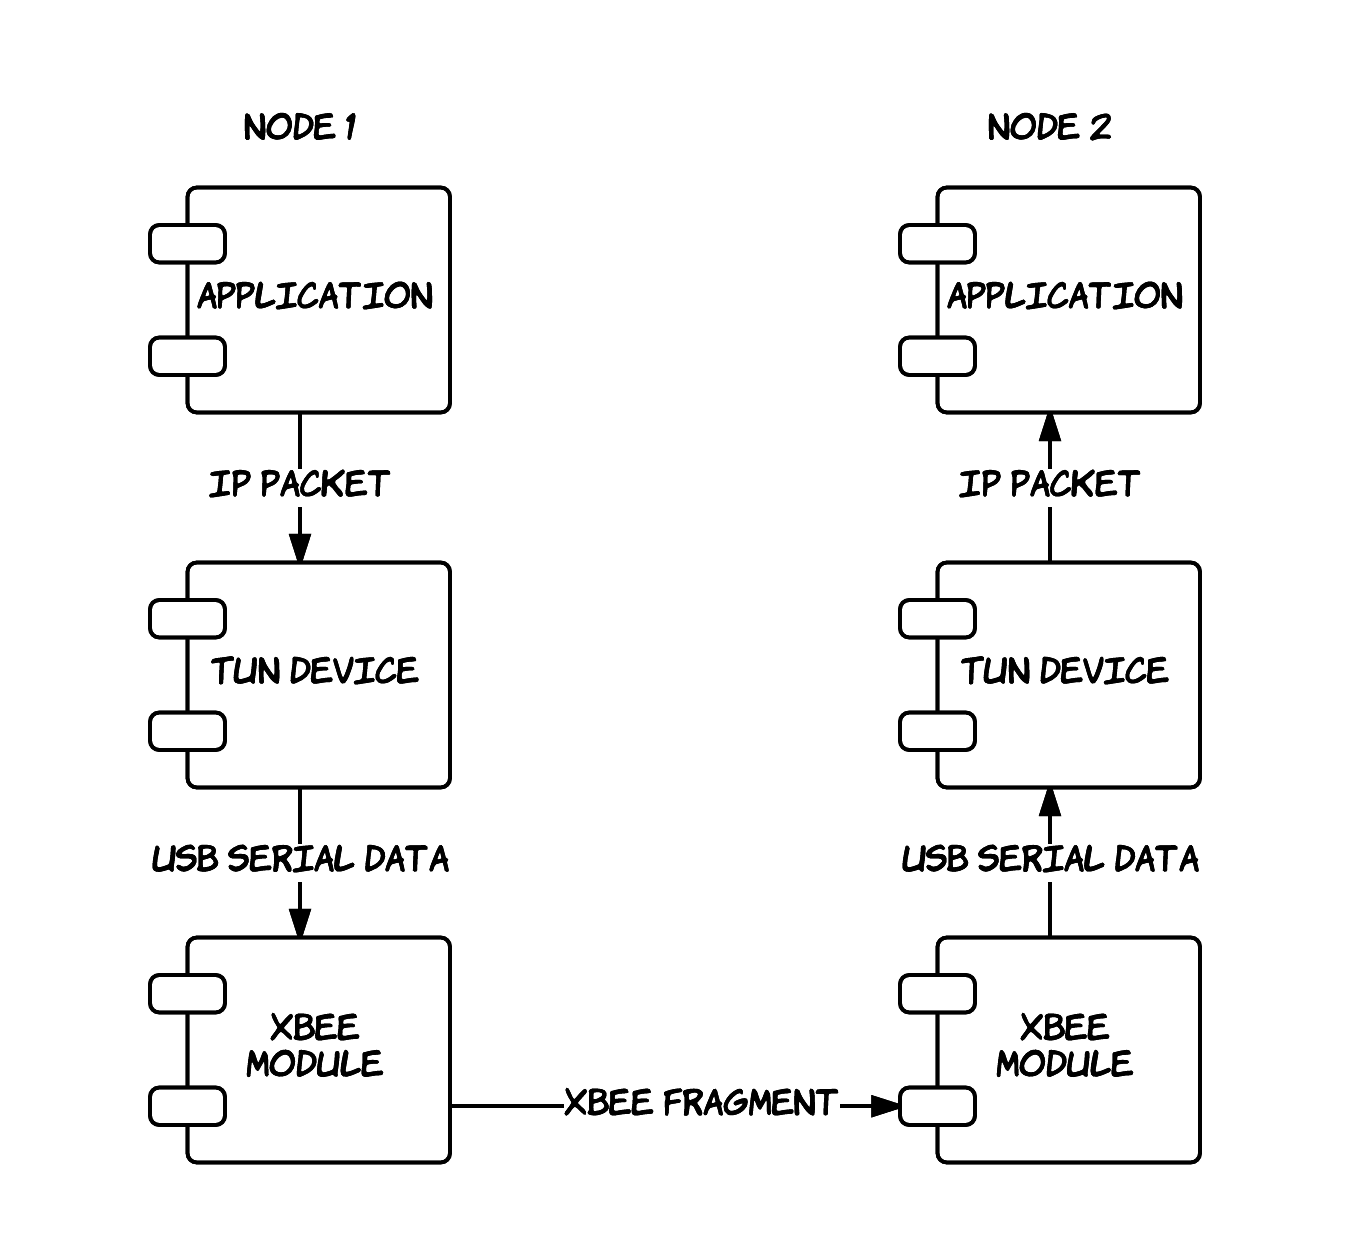
\includegraphics[scale=.9]{xbee_subsystems.png}
\caption{Data is sent from Node 1 to Node 2 through the various subsystems}
\label{fig:xbee_subsystems}
\end{figure}

In Figure~\ref{fig:xbee_system_distribution}, we show the network components and their subsystems, as well has the protocols used to communicate between the subsystems. Note that data at each layer of the network is virtualized such that each subsystem's behaviour and data processing does not need to be modified. In other words, applications on each node operate exactly as they would on a normal Internet connection.

\begin{figure}[htbp]
\centering
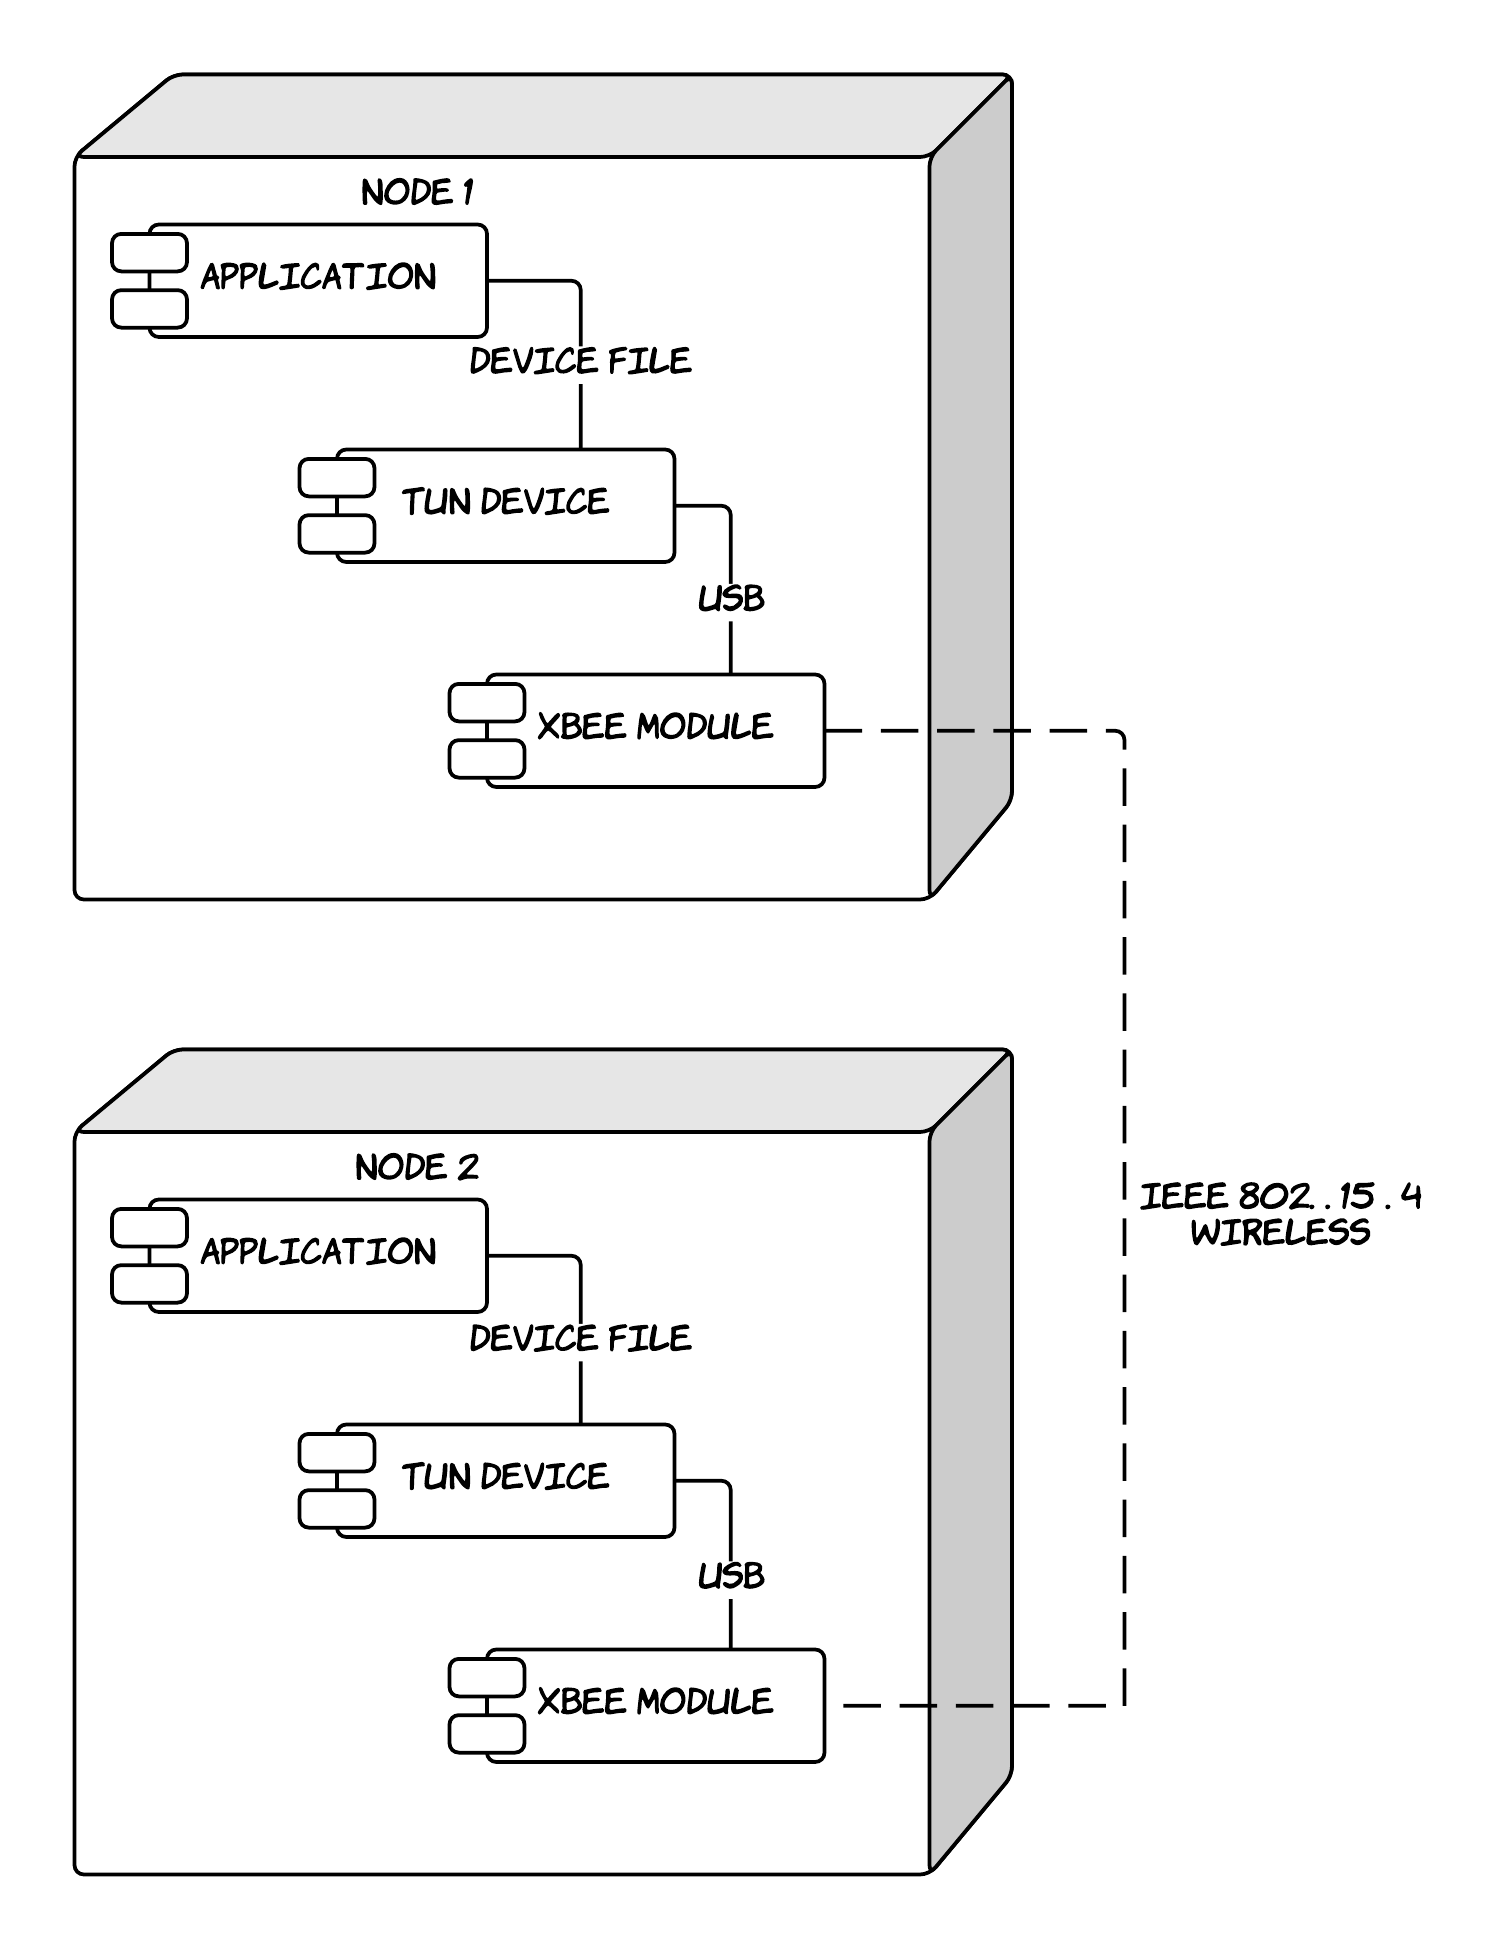
\includegraphics[scale=.9]{xbee_system_distribution.png}
\caption{Component distribution in the XBee-based network}
\label{fig:xbee_system_distribution}
\end{figure}

\subsubsection{XBLink}

To enable quick setup of the XBee-based network between two computers, we have developed a program called XBLink to create a TUN device, and handle the communication from applications on the node to the XBee modules. The C++ program is compiled using g++, and runs under standard Linux systems with access to /dev/net/tun and /dev/urandom.

Once the program is compiled, it is run as follows, with a number of command line arguments:
\begin{verbatim}
./xblink usb_dev xbee_model baud addr tun_dev
\end{verbatim}

The argument usb\_dev is the path to the XBee USB device; xbee\_model refers to the specific type of XBee module used; baud refers to the baud rate preset on the XBee module; adde refers to the destination address of the XBee module on the \textit{other} node; and tun\_dev is an user-chosen name to assign to the TUN device to be created.

As a specific example, we create a TUN device named ``tun77", using the following command:
\begin{verbatim}
./xblink /dev/ttyUSB0 xbeeZB 115200 0x0013A200409E0550 tun77
\end{verbatim}
Here, our XBee USB adapter is located at /dev/ttyUSB0; our XBee model is ZB; the baud rate has been set at 125200; and the address of the XBee module that we're connecting to is at $0x0013A200409E0550$. Note that the XBLink program runs for the duration of the connection, and outputs useful data, such as XBee fragment info.

Once the TUN device is created and running, we must assign an IP address to it. This is done by first enabling the device as a network interface:
\begin{verbatim}
sudo ip link set tun77 up
\end{verbatim}
This Linux command simply activates the TUN device that we have created as a network interface. Next, we assign an IP address range to it:
\begin{verbatim}
sudo ip addr add 10.0.0.2/24 dev tun77
\end{verbatim}
This command assigns the IP addresses 10.0.0.2/24 to the TUN device. Now, all internet traffic that is routed through this address range will be accessed through the TUN device. For example, if we ping the address, then UDP packets will be sent through the device to the other computer. This means that we have now successfully connected our nodes over the network.

In this section, we have described the system components in our implementation, and outlined the procedures of setting up the XBee-based network. In section~\ref{subsec:config}, we describe the way that the XBee modules have been configured to work effectively in our system.

\subsection{Configuration of XBee Modules}
\label{subsec:config}

********************************************

*****************************************

***************************************

\subsection{Sample Usage}
\label{subsec:usage}

\subsubsection{Network Applications}
In this section, we give some examples of usage of our system. First, we simply ping the other node, using Linux's built in ping command, shown in Figure~\ref{fig:xblink_ping}. In this figure, we see the result of ping, with some statistics on packets sent, and transmission speed. In this example, each packet had a size of 72 bytes (plus header), no packets were lost, and 100 pings required a total time of about 1.5min.
\begin{figure}[!ht]
\centering
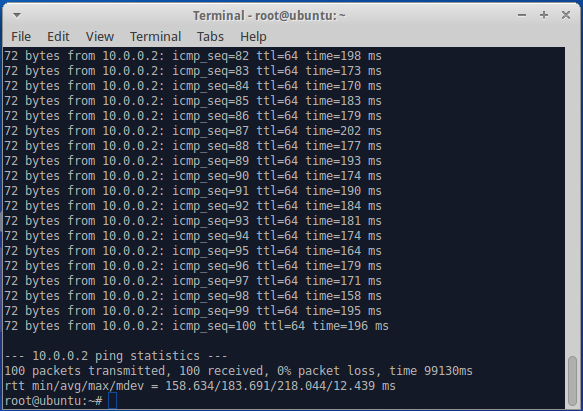
\includegraphics[scale=.6]{xblink_ping.png}
\caption{Running the program ping over the network}
\label{fig:xblink_ping}
\end{figure}

In Figure~\ref{fig:xblink_console}, we see the output of the XBLink program during execution of the ping program, which displays information about sent and received fragments and packets. In this example, packets only needed to be split over two fragments, as expected, since two fragments can contain a total payload size of 128 bytes. 
\begin{figure}[!ht]
\centering
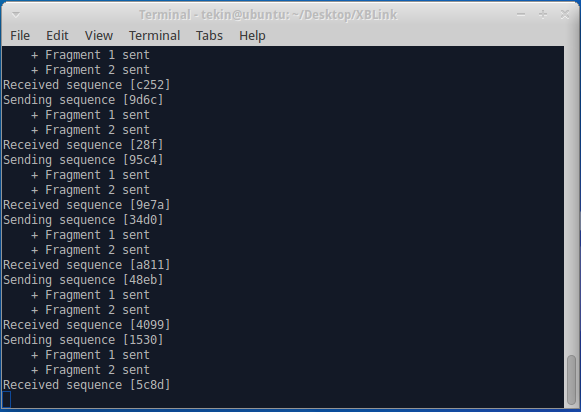
\includegraphics[scale=.6]{xblink_console.png}
\caption{Console output of the XBLink program during a network connection}
\label{fig:xblink_console}
\end{figure}

We are also able to perform secure file transfers between the two nodes. Figure~\ref{fig:xblink_sftp} shows the successful transfer of a 19KB file over SFTP, at a data rate of about 1KB/s. We were able to run the program using default setup, without adjustments for the slower transmission speeds.
\begin{figure}[!ht]
\centering
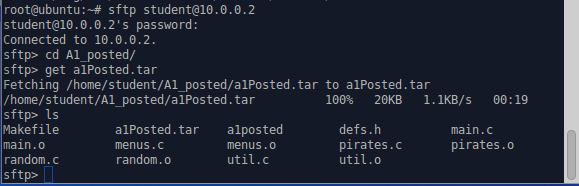
\includegraphics[scale=.6]{xblink_sftp.png}
\caption{Transferring a file over SFTP}
\label{fig:xblink_sftp}
\end{figure}

Finally, we show that we are able to create a secure connection from one node to the other, using SSH. Figure~\ref{fig:xblink_ssh} shows that we are able to login to the other node under the ``student" account, and view the home directory. Of course, this is not a surprise, since we were able to perform secure file transfers using SFTP, which uses SSH as the underlying protocol.
\begin{figure}[!ht]
\centering
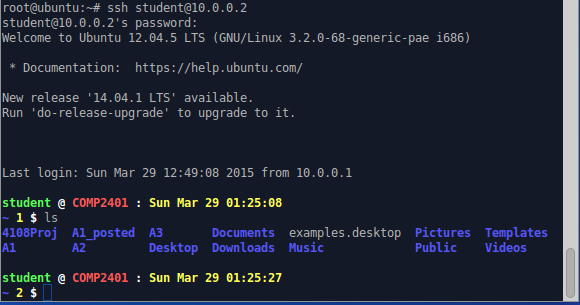
\includegraphics[scale=.6]{xblink_ssh.png}
\caption{Logging in to a remote node using SSH}
\label{fig:xblink_ssh}
\end{figure}

\subsection{Simple Performance Analysis}
To gain a rough idea of the performance of the XBee network, we perform a number of ping operations at different packet sizes, and analyze the data rates for each packet size. Figure~\ref{fig:xbee_performance} shows the various packet sizes used, in bytes, and the required average roundtrip time. The figure also shows, for the pings, the percentage of packets that were lost during transmission.
\begin{figure}[!ht]
\centering
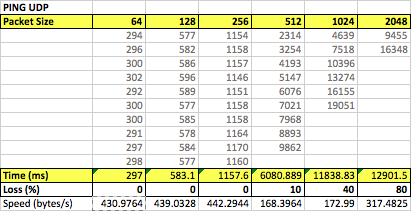
\includegraphics[scale=.8]{xbee_performance.png}
\caption{A comparison of data transfer performance under different conditions}
\label{fig:xbee_performance}
\end{figure}

From the figure, we immediately notice that higher number of packets were lost for larger packet sizes. It is possible that the ping program does not wait long enough for the XBee modules to send all the fragments of the packet, and erroneously considers the packets lost. It is also interesting that the transmission durations appear to increase over time, for larger packet sizes. This further supports the hypothesis above, since the modules have not completely transmitted all of the fragments in the first packet, before another packet is queued.

Disregarding measurements with packet losses, we see that the computed average data transfer rate is about 440B/s. However, this does not consider that there are extra headers in each packet, which can significantly increase the data size for small packets. Either way, we see that the data rate is relatively steady for all packet sizes below 256B. 

Thus, we have presented examples of how our system can be used for basic Internet networking, and analyzed the performance of the network. Next, we summarize our achievements and conclude the report.

\section{Summary}
\label{sec:summary}

For this project, we have designed and implemented a text-based Hangman game that can be played by multiple players over an internet network. The data sent between the client and server nodes are Byte-sized, and the information is encrypted using a Simplified Data Encryption Standard algorithm. The program is designed using Java, and runs on any computer with a current version of the Java Runtime Environment. Connection between client and server is established using a stream socket implementation, which adequately suits our data transmission requirements.

\subsection{Possible Future Directions}
As mentioned above, our system is designed to accommodate up to two players connecting to each host. However, it would be easy to extend the design to accommodate a much larger number of players. Further, it is possible to use the same system design to implement a multiplayer networking version of a different game, such as the card game solitaire, or Yahtzee, etc. It would also be possible to extend the server design to allow close interactions between each client; this would allow further possibilities in providing additional game types to the users.

It would also be possible to use a more powerful encryption algorithm, in conjunction with a mode of operation such as Counter Mode, to increase the security of the data transmission. There are a number of widely available libraries for various programming languages and environments. We have implemented our own version of S-DES here as an academic exercise.

\newpage
\bibliography{rep_ref}
\bibliographystyle{unsrt}

\end{document}